\chapter{Background}\label{chapter-background}
The first section of this chapter, terminology \ref{section-terminology}, explains terms that are used throughout this thesis. The next section, Android development methods \ref{section-android-development-methods}, explains different methods of developing an Android mobile application. The following section, lines of code \ref{section-lines-of-code}, describes lines of code as a software metric and what it measures. Lastly, the section related work \ref{section-related-work}, suggests related work to this thesis for further reading. 

\section{Terminology}\label{section-terminology}
\begin{description}
  \item[Mobile application] \hfill \\
    Refers to the application being developed, excluding code loaded from remote websites.
  \item[Web application] \hfill \\
    If nothing else is specified it refers to the client-side of the web application.
  \item[Development methods] \hfill \\
    Refers (in the context of this paper) to the methods of mobile application development methods being evaluated. I.e developing the mobile application with PhoneGap or natively in Android.
  \item[Native function] \hfill \\
     A hardware function which a device has. Lets say a mobile has a camera and an accelerator. When writing software for that mobile there are functions to interact with the camera and accelerator. Those functions are called native functions.
  \item[Web/Mobile application layer] \hfill \\
	Refers to the application layer belonging specifically to the mobile application or the web application. A mobile application can encapsulate a web application which then is a a part of the mobile application. The mobile application then consists of a mobile and web application layer.
	\item[Native application] \hfill \\
	A native application is an application that is developed to be used on a particular device or plattform. For example, a native application for Android is an application that is written to run on the Android operating system.
\item[Web technologies] \hfill \\
	In the context of this paper, web technologies refer to languages used when developing web applications, such as HTML, CSS and JavaScript.
\item[Hybrid application] \hfill \\
	A hybrid application is a native application which is partially written with web technologies. The part of the application written with web technologies runs within a browsers engine. The browser engine in Android is called WebView. A web application running in a web browser on a mobile does not have access to the mobiles native functions such as the accelerometer. However, a web application running within a WebView can access a device native functions. 
\end{description}

\section{Android development methods}\label{section-android-development-methods}
Android is an operating system used on a wide range of devices \cite{dell2011}. For example a mobile device or tv device. Android applications are usually developed in the programming language Java using the Android SDK.

A software library for a system is a set of functions which can be used when developing applications for that system. A framework is a layered structure to help or simplify for the developer to develop software for a system. A framework differs from a library in the following way \cite{riehle2000}:

\begin{itemize}
\item The program's flow of control is dictated by the framework instead of the caller
\item A framework has a useful default behavior
\item The framework can be extended by the user
\end{itemize}

\subsection{Android application framework} 
The Android SDK includes a set of tools \cite{sdk2015}. Tools such as virtual device tools, development tools, debugging tools and buid tools. An Android application that is developed natively is an application that is developed using the Android SDK. The year 2012 60\% of all open source developers writing Android or IOs applications only used the official SDK \cite{eclipse2012}. For developing Android applications Android provides an application framework \cite{android-framework2015}. Some important classes from the Android SDK, used in the application developed for this thesis, are presented below.

\subsubsection{Activity}\label{sec:activity}
According to Androids developer site \cite{activity2015} "An Activity is a single, focused thing that the user can do.". In it's most simple form, an Android application consists of a single Activity, in charge of creating the window to render the application UI and interact with the user. Another example of a simple Activity is when requesting an image from the camera through another application. An Activity can be started with the use of an Intent, see below, and as soon as the Activity has finished it's task (an image has been captured), it is terminated and the result is sent back to the parent Activity.

\emph{Example. Starting an Activity for result using an Intent}
\begin{lstlisting}
// In MainActivity
// Create Intent
Intent intent = ...

// Start activity based on intent
startActivityForResult(intent, some_request_code)

// When activity is completed, handle the returned data
onActivityResult(requestCode, resultCode, data){
// Do something with data depending on request/result code
}
\end{lstlisting}

\subsubsection{Intent}
According to the Android Developers site \cite{intent2015} "An intent is an abstract description of an operation to be performed.". In this paper, Intents are only used as a means to request data from native Android functions, such as the mobile camera.  

\subsubsection{WebView}
A WebView \cite{webview2015} is a View \cite{view2015} that can be used to render web content inside of an application. The application can invoke JavaScript in the WebView, but JavaScript in the WebView has no way of accessing the Java objects of an application. This can however be changed by exposing a Java Object with the use of JavaScriptInterface, see below.

\subsubsection{JavaScriptInterface}
Allows exposing methods to JavaScript, by exposing a Java Object annotated by the @JavaScriptInterface tag. The JavaScriptInterface is added to a single WebView through the addJavaScriptInterface method, and is thus only exposed to JavaScript running in this WebView. For further reading, refer to the Android Developers site \cite{jsi2015}.

\subsection{Development frameworks for Android applications}
Android has undertaken 15 powerful, open source and cross platform frameworks. The frameworks are usually aimed at web developers and are developed using web technologies \cite{mondal2013}.

\begin{itemize}
\item PhoneGap
\item JQuery mobile
\item Sencha Touch
\item Dojo Mobile
\item Titanium
\end{itemize}

After using the Android SDK the most widely used mobile framework for Android is JQuery mobile and PhoneGap. In 2012 28.6\% used JQuery mobile and 17.9\% used PhoneGap \cite{eclipse2012}. The frameworks listed above support Android and IOs but often target other platforms such as Blackberry and Windows Phone as well \cite{mondal2013}. 

\subsection{PhoneGap}
PhoneGap is developed with web technologies. The code can be compiled to different platforms, such as Android or IOs specific code. The resulting application is a hybrid application. An example of a mobile application built in PhoneGap is Wikipedia's mobile application.

One of the huge advantages developing in PhoneGap compared to developing using the Android SDK is that PhoneGap can be compiled to multiple platforms, see figure \ref{figure-phonegap-plattoforms}. Making PhoneGap an attractive development framework for companies with less development resources. If a mobile application is developed natively for Android, IOs and Windows Phone, maintaining the mobile application must be done in three different native applications. If the mobile application is instead developed in PhoneGap only one application needs to be maintained.

\begin{figure}\label{figure-phonegap-plattforms}
\centering
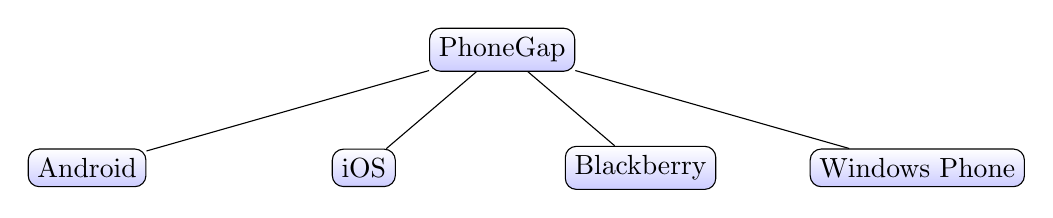
\begin{tikzpicture}[sibling distance=10em,
  every node/.style = {shape=rectangle, rounded corners,
    draw, align=center,
    top color=white, bottom color=blue!20}]]
  \node {PhoneGap}
    child { node {Android} }
    child { node {iOS} }
    child { node {Blackberry} }
    child { node {Windows Phone} };
\end{tikzpicture}
\medskip
\caption{PhoneGap can be compiled into multiple plattoforms.} 
\end{figure}

A disadvantage of developing in PhoneGap is when there is a use of many native features. PhoneGap relies on a development framework and the provided features when building a mobile application. Hence, if the framework is not up to date with the latest new features, the developer will not be able to partake of the features until the framework is updated. If the application is dependent on many native features a hybrid application may have limitations\cite{kohan2015}.

\subsection{Inline frame}
An inline frame, is used to embed another document within the current HTML document. Communication from the parent document to the document inside the inline frame, is easily implemented since it has direct access to the window and can invoke JavaScript functions in the inline frame. Communicating the other way however requires more preparations. An example how to solve it is using the postMessage method of the parent window, and implementing a message listener.

\subsection{JQuery mobile}
%here we'll write about jquery mobile framework

\section{Lines of code}\label{section-lines-of-code}
Source lines of code is a measurement tool for software development. Source lines of code, also abbreviated as SLOC, is very easy to obtain and is a fairly accurate predictor of development effort\cite[p.~63]{galorath2006}. Measuring SLOC simply means you count the number of lines of code. There are many different ways to measure SLOC, such as Halsted’s approach, function points, physical SLOC and Logical SLOC. 

Physical SLOC is the length of the code excluding comments and blanks. Function points measure functionality and can therefore be measured before the design and coding if the requirement specification is complete\cite[p.~187]{galorath2006}. Halstead’s uses measurable properties such as operands and operators and uses them to identify properties of software. Such as the length, difficulty and effort of the program. Fenton and Bieman describes Halstead’s software science measures as a confused and inadequate measurement. Particularly for other attributes then size\cite[p.~345]{fenton2015}.

Logical SLOC measures the number of statements that carry over one or more physical lines.  For languages with terminators, this can be counted more easily and quickly. As an example, in Java you could count the logical SLOC by counting the number of line-terminating semicolons and closing curly brackets. Logical SLOC represents the programming instructions and data declarations which are converted into executable instructions, i.e. the implementation of the software design. Another positive aspect of of logical SLOC is that it better handles differences in formatting and style conventions than physical SLOC\cite[p.~155]{galorath2006}.

To compare size between two different languages a size conversion table can be used. The table can be used to estimate how many SLOC a program coded in one programming language would have in another language. In the table constructed by Galorath and Evans you can compare a third generation language, a fourth generation language, Ada, Assembly or Pascal\cite[p.~163]{galorath2006}. A third generation language compared to another third generation language would have no conversion rate. 

Source lines of code is a measurement tool for software development. Source lines of code, also abbreviated as SLOC, is very easy to obtain and is a fairly accurate predictor of development effort\cite[p.~63]{galorath2006}. Measuring SLOC simply means you count the number of lines of code. There are many different ways to measure SLOC, such as Halsted’s approach, function points, physical SLOC and Logical SLOC. 

Physical SLOC is the length of the code excluding comments and blanks. Function points measure functionality and can therefore be measured before the design and coding if the requirement specification is complete\cite[p.~187]{galorath2006}. Halstead’s uses measurable properties such as operands and operators and uses them to identify properties of software. Such as the length, difficulty and effort of the program. Fenton and Bieman describes Halstead’s software science measures as a confused and inadequate measurement. Particularly for other attributes than size\cite[p.~345]{fenton2015}.

Logical SLOC measures the number of statements that carry over one or more physical lines.  For languages with terminators, this can be counted more easily and quickly. As an example, in Java you could count the logical SLOC by counting the number of line-terminating semicolons and closing curly brackets. Logical SLOC represents the programming instructions and data declarations which are converted into executable instructions, i.e. the implementation of the software design. Another positive aspect of of logical SLOC is that it better handles differences in formatting and style conventions than physical SLOC\cite[p.~155]{galorath2006}.

To compare size between two different languages a size conversion table can be used. The table can be used to estimate how many SLOC a program coded in one programming language would have in another language. In the table constructed by Galorath and Evans you can compare a third generation language, a fourth generation language, Ada, Assembly or Pascal\cite[p.~163]{galorath2006}. A third generation language compared to another third generation language would have no conversion rate. 

\section{Related work}\label{section-related-work}
% if anyone asks for a deeper research or surroundin topic here the work that we can reco

\iffalse
%not really sure what to do with this section. I think actually might belong in approach
\subsection{Development goals} \label{subsection-development-goals}
Antoher goal is that the mobile application only provides data from native functions. In order to achieve that the web application and mobile application should have a master slave relationship. Where the web application acts as the master and the mobile application as the slave. To get data from the mobiles native functions the web application asks for the data and the mobile application passes the data back.

To enable this master and slave relationship the mobile and web application layer must be able to communicate. Passing commands and data between the layers. It is important the mobile and web application layers has a way of communicating that is developer friendly. 

It is important that the logic of the web application can be written in a general way (non-platform dependant) adapting to the device accessing the web application. So that the same web application code is used for the web application and mobile application.
\fi